\documentclass{article}

\usepackage{titlesec}
\usepackage{titling}
\usepackage{url}
\usepackage[margin=.5in]{geometry}
\usepackage{xcolor}
\usepackage{lipsum}
\usepackage{setspace}
\usepackage{listings}
\usepackage{caption}
\usepackage{graphicx}
\usepackage{ulem}
\usepackage{enumitem}
\usepackage{hyperref}

\title{FastAPI from a CRUDmaker's POV: A Start-to-Finish Example}
\author{Daniil Kraynov -- \href{https://parkanaur.net}{parkanaur.net}}

% Text/list formatting
\hypersetup{colorlinks=true, urlcolor=blue}
\onehalfspacing
\setlist{noitemsep}
\newcommand{\sectionbreak}{\clearpage}
%\setcounter{tocdepth}{4}
\setcounter{secnumdepth}{3}

\titleformat{\paragraph}
{\normalfont\normalsize\bfseries}{\theparagraph}{1em}{}
\titlespacing*{\paragraph}
{0pt}{3.25ex plus 1ex minus .2ex}{1.5ex plus .2ex}

% URL footnotes and some text macros
\newcommand{\flink}[1]{\footnote{\href{#1}{#1}}}
\newcommand{\note}{\textbf{\color{red}Note: }}
\newcommand{\optional}{{\rmfamily\bfseries\color{gray} [optional] }}

% Generic code listing style - c means code, not C
\definecolor{darkgreen}{RGB}{0, 100, 0}

\lstdefinestyle{cstyle}{
    numbers=left,
    basicstyle=\ttfamily\small,
    commentstyle=\color{darkgreen}\small,
    keywordstyle=\color{blue}\bfseries,
    showstringspaces=false,
    aboveskip=0.5cm,
    xleftmargin=0.5cm,
    framesep=0mm,
    frame=tb,
    framexleftmargin=0.75cm,
    columns=fullflexible,
    breaklines=true}

\captionsetup[lstlisting]{margin=0cm}
\renewcommand{\lstlistingname}{File}
\renewcommand{\lstlistlistingname}{List of \lstlistingname s}

% Generic code listings
\lstnewenvironment{code}[2][]{\lstset{language=#1, caption=#2, style=cstyle, escapeinside={(*@}{@*)}}}{}
\newcommand{\cinline}[2]{{\lstinline[language=#1, style=cstyle, basicstyle=\ttfamily\normalsize]{#2}}}

% Python code listings
\lstnewenvironment{pycode}[1][]{\lstset{language=Python, caption=#1, style=cstyle, morekeywords={async}, escapeinside={(*@}{@*)}}}{}
\newcommand{\pyinline}[1]{\lstinline[language=Python, style=cstyle, morekeywords={async}, basicstyle=\ttfamily\normalsize]{#1}}

% Bash code listings
\lstnewenvironment{bashcode}[1][]{\lstset{language=bash, caption=#1, style=cstyle, morekeywords={docker, poetry, git, mv, python, uvicorn}, escapeinside={(*@}{@*)}}}{}
\newcommand{\bashinline}[1]{\lstinline[language=bash, style=cstyle, morekeywords={docker, poetry, git, mv, python, uvicorn}, basicstyle=\ttfamily\normalsize]{#1}}

% Docker code listings
\lstdefinelanguage{docker}{
    basicstyle=\ttfamily\small,
    keywords={FROM, RUN, COPY, ADD, ENTRYPOINT, CMD,  ENV, ARG, WORKDIR, EXPOSE, LABEL, USER, VOLUME, STOPSIGNAL, ONBUILD, MAINTAINER,
    image, environment, ports, container\_name, ports, links, build, version, volumes, services, networks},
    keywordstyle=\color{blue}\bfseries,
    identifierstyle=\color{black},
    sensitive=false,
    comment=[l]{\#},
    commentstyle=\color{darkgray}\small
}
\lstnewenvironment{dockercode}[1][]{\lstset{language=docker, caption=#1, style=cstyle, escapeinside={(*@}{@*)}}}{}
\newcommand{\dockerinline}[1]{\lstinline[language=docker, style=cstyle, basicstyle=\ttfamily\normalsize]{#1}}

\begin{document}

\maketitle

% TOC
{\hypersetup{linkcolor=black}
\tableofcontents}

\section{Introduction}

FastAPI, a high-performant Python web framework, is very well documented, but the documentation might be a bit too overwhelming for a semi-seasoned developer who already has experience with designing web applications and has a general stance on how they should be structured.

I've started writing this article as a compilation of notes to refer to when writing an app in FastAPI from the ground up. The end result of my initial tinkering with FastAPI, documented here, is a file hosting application with a bunch of extras like Docker integration.

Due to FastAPI being an ASGI framework, deployment process is a little bit different from using nginx and uWSGI, so I hope to cover the deployment caveats as well.

\subsection{Who is this article intended for}

This article aims to help developers coming from other frameworks (Flask, Django, as well as non-Python ones) who know what they're doing and are willing to jump straight into action but don't feel like getting overwhelmed with deeper aspects of FastAPI's official documentation \flink{https://fastapi.tiangolo.com} (I still advise everyone to read it - it's good on its own and is quite helpful!).

It could also be of good use to beginner developers, but some aspects of this article \textit{might} be harder to understand for them - please give feedback on whether it's a good read or not!

\subsection{Application building steps}

From my experience, the general workflow for producing a mid-sized web application is as follows:

\begin{enumerate}
    \item Designing a set of domain model classes (e.g. User, Item, etc.)
        \begin{enumerate}
            \item Choosing a data source
            \item Likely some automatic migration scripts
        \end{enumerate}
    \item Creating an API skeleton for at least one entity
        \begin{enumerate}
            \item Authentication logic
        \end{enumerate}
    \item Adding a business logic layer for at least one entity
    \item Binding it all together
    \item Adding logic/API for the rest of the entities
    \item \optional Adding a frontend and a bunch of non-logic pages (in parallel with the previous steps or after them, depending on size of the developing team)
    \item \optional Deploy scripts, tests, CI/CD, etc.
\end{enumerate}

FastAPI's documentation describes or mentions most of these steps, but in no specific order. For an experienced developer there are pages of particular interest (e.g. app structure for bigger applications \flink{https://fastapi.tiangolo.com/tutorial/bigger-applications/}, but from there you have to go deeper into the documentation in order to find out how to structure your models, DTOs, etc.

You'd probably start jumping around more and more around the documentation, get overwhelmed with the amount of points (most likely you wouldn't need all of them at the start of your FastAPI journey), and, in the worst case, lose motivation in learning FastAPI - it happened to me at first, which is a shame, because FastAPI is a beautiful framework!

\subsection{Feedback}

I don't consider myself an expert in either programming, documentation, or English, and this article is certain to have bad architecture decisions or mishaps in general.

I encourage you to send your comments regarding this article, whether they're about me doing a good job or being an ignorant fool who doesn't know any better (I'm serious on this one!). Maybe you can think of a few additions as well, in which case you can also fork this article - it's "licensed" under CC0, so you're free to do whatever you want with it.

You can send your comments via GitHub issues/PRs \flink{https://github.com/parkanaur/fastapi-notes} or by sending an e-mail at {\href{mailto:dan@parkanaur.net}{dan @ parkanaur.net}}. Don't hesitate!

\section{Preparations}

The project that I'm going to describe is \textbf{PyFH} \flink{https://github.com/parkanaur/pyfh}, a file hosting application designed for self-hosting, with a few additional features like public/private files, timed files, encryption, etc.

I'll try to follow the incremental model, starting at the very basic things like setting up environment all the way to deployment on a real world VPS.

\subsection{Setting up environment}

It seems that the good old requirements.txt is slowly falling out of favor within the Python ecosphere, so we're gonna \sout{bite the bullet} follow suit and use the newer toolset (i.e. Poetry). This is a good exercise in using non-standard tooling as well.

Poetry is supposed to make managing virtualenvs and dependencies easier, so let's go ahead and install it \flink{https://python-poetry.org/docs/}.

You can use regular requirements.txt instead - be sure to remove Poetry-related lines and replace them with manual venv creation (\bashinline{python -m venv venv}).

\begin{bashcode}
# Poetry will create the project directory for you automatically
cd ~/code
poetry new pyfh
cd pyfh
git init

# Virtualenv creation/activation (deactivate with exit)
poetry shell

# Don't @ me
mv README.rst README.md
\end{bashcode}

Time to add dependencies. We're building a file hosting app, so we're gonna need a few extras for our FastAPI dependency. It's a good idea to just add the whole \texttt{fastapi[all]} dependency during development - it adds multipart support, as well as a few more goodies, and if you care about the amount of your dependencies, you can clean the unneeded stuff out later.

\texttt{fastapi[all]} also installs \texttt{uvicorn[standard]} as per FastAPI installation tutorial.

\note Most of the bash commands will imply that you have activated your virtualenv (\bashinline{poetry shell}).

\begin{bashcode}
# Install our dependency - same as (pip install + freeze > requirements.txt)
# If you're using zsh, enclose fastapi[all] in quotes
poetry add fastapi[all]
\end{bashcode}

Now we're ready to start adding more stuff into the project.

\subsection{Initial project structure}

First we have to add some boring stuff - a few folders with empty \texttt{\_\_init.py\_\_}'s in them, a barebones main.py file, .gitignore, etc.

\subsubsection{\texttt{main.py}}

This is similar to \texttt{main.py/wsgi.py} in Flask - an ASGI server will use it as a starting point for your application (same as passing \texttt{main:app} to uWSGI, if you will).

Let's add the simplest \texttt{main.py} possible for now:

\begin{pycode}
from fastapi import FastAPI

app = FastAPI()

@app.get("/")
async def test():
    return "Welcome to pyfh!"
\end{pycode}

Note the \pyinline{async} keyword - it's used extensively in FastAPI. Asynchronous programming is a topic which isn't covered extensively in this article, but what you should know is that in most of the cases it really speeds things up. It is native to FastAPI development, in particular to path operations (\pyinline{fastapi.get(), .post()}, etc.) - read more at the official documentation \flink{https://fastapi.tiangolo.com/async/}.

Let's try the code out. Uvicorn is used to launch ASGI apps \flink{https://www.uvicorn.org/deployment/} (we'll cover production deployment later), \texttt{--reload} enables auto-restart on code changes:

\begin{bashcode}
uvicorn main:app --reload
# ..... ^^^^---- main.py
# ..... -----^^^ app = FastAPI()
\end{bashcode}

Alternatively you can call \texttt{uvicorn.run()} in main.py, rather than use the command-line tool.

Then make an HTTP request to 127.0.0.1:8000 and you should see something along the lines of the following:

\begin{figure}[h]
    \centering
    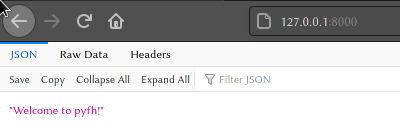
\includegraphics[width=0.7\textwidth]{img/helloworld.png}
    \caption{Hello World in FastAPI}
\end{figure}

\subsubsection{Folders and \texttt{\_\_init.py\_\_'s}}

Time to add some more structure. Files not in the root directory \textbf{are empty} unless otherwise noted. To save time, I'll assume you know what \texttt{\_\_init.py\_\_'s} are for.

{\ttfamily
\begin{itemize}
    \item $\sim$/code/pyfh
        \begin{itemize}
            \item main.py
            \item pyproject.toml
            \item poetry.lock
            \item .gitignore
            \item README.md
            \item \optional .env
            \item Dockerfile *
            \item .dockerignore *
            \item docker-compose.yml *
            \item pyfh/
                \begin{itemize}
                    \item \_\_init.py\_\_
                    \item config.py
                    \item entities/
                        \begin{itemize}
                            \item \_\_init.py\_\_
                            \item user.py
                        \end{itemize}
                    \item{routes/}
                        \begin{itemize}
                            \item \_\_init.py\_\_
                            \item user.py
                        \end{itemize}
                \end{itemize}
        \end{itemize}
\end{itemize}
}

* You may have noticed the presence of Docker-related files. We'll put Docker to good use in the next section. As much as I hate to admit it, Docker's just too useful sometimes.

\subsubsection{\texttt{gitignore}}

Github's Python gitignore will do just fine \flink{https://github.com/github/gitignore/blob/master/Python.gitignore}, but read the notes below.

\note You don't need to add \texttt{poetry.lock} to .gitignore - it's used to freeze currently installed (on your machine) package versions (similar to versions in \texttt{requirements.txt}). Poetry will make use of that file on other developers' machines to produce the same environment you have. You can later run \bashinline{poetry update} to use newer package versions.

\note Be sure to add \texttt{.env} to your .gitignore if you follow the structure above. We'll only use that .env file for development purposes, and it's generally \textbf{not recommended} to keep configuration data inside your codebase. When preparing your code for production deployment, make sure to keep .env files in a secure location.

\subsection{Configuration files}

I firmly believe that for a project with more than a few files of code it is important that you deal with configuration and deployment details as early as possible.

Setting up proper configuration for your project can be hard, especially if you want it to be easy to use in production later on and have little experience in starting projects from scratch.

\subsubsection{Environment variables}

It is common practice to use \textbf{environment variables} as configuration source for applications. They're used extensively in Docker and Docker Compose too.

In Linux, env variables are set the following way:

\begin{bashcode}
export VAR_NAME="var_value"
export VAR_INT_VALUE=12
\end{bashcode}

In Python you read them the following way:

\begin{pycode}
import os
# default value argument is optional
var_name = os.getenv("VAR_NAME", "default value") # -> "var_value"
var_int_value = os.getenv("VAR_INT_VALUE") # -> "12" <- note that os.getenv always returns a string
\end{pycode}

It is also common to write \textbf{env files} (prefixed with dot: \textbf{.env}) to store environment variables in. You may have noticed files that look like this when working with Docker images:

\begin{bashcode}[\texttt{.env} (example)]
    VAR_NAME=var_value
    VAR_INT_VALUE=12
\end{bashcode}

\subsubsection{Managing configuration in FastAPI with Pydantic \label{preparations:configenv}}

You could make use of \pyinline{os.getenv}, but FastAPI docs suggest a different way, and it's much more elegant.

FastAPI utilizes at its core Pydantic, a data validation library, to check what's coming from users. It is also used for settings management \flink{https://pydantic-docs.helpmanual.io/usage/settings/}, and it makes working with configurations a breeze.

We have created a separate \textbf{config.py} for managing project configuration - let's use it. Right now we only need database info - the rest will be added as needed.

\begin{pycode}[\texttt{pyfh/config.py}\label{config.py1}]
from pydantic import BaseSettings


class Settings(BaseSettings):
    db_host: str = "127.0.0.1"
    db_port: int = 5432

    # Nested "Config" classes are used by Pydantic classes for additional base classes configuration,
    # e.g. env file location for BaseSettings / orm mode usage for Pydantic models (BaseModel)
    class Config:
        env_file = ".env"
        #case_sensitive = False

settings = Settings() (*@ \label{config.py1:si} @*)
\end{pycode}

All required environment variables are then read by Pydantic when \pyinline{Settings} is initialized as a variable on line \ref{config.py1:si}.

\note Pydantic reads environment variables in a \textbf{case-insensitive} way. In the following file, both variables are eligible to be read into the class above:

\begin{bashcode}[\texttt{.env}]
db_host=10.0.12.23
DB_PORT=5000
\end{bashcode}

You can change that behavior by uncommenting the line in the \pyinline{Settings.Config} class.

The order in which Pydantic reads environment variables is as follows:

\begin{enumerate}
    \item If defined, exported (not in the \textbf{.env}) variables are used
    \item If defined, the \textbf{.env} variables are used
    \item Fallback to default values (127.0.0.1 and 5432 in our case)
\end{enumerate}

That means \bashinline{export DB\_HOST=10.0.0.1} will take precedence over \bashinline{DB\_HOST=127.0.0.1} from \textbf{.env}.

\note If you're using development and/or deployment via Docker/Docker Compose, you most probably \textbf{don't} need to use env file configuration in a Pydantic class - in this case environment variables are defined and passed to the application using Docker commands - see Section \ref{preparations:dockerenvs}

If you still have questions, read up on official FastAPI docs for settings management, which should answer them all \flink{https://fastapi.tiangolo.com/advanced/settings}.

\subsection{Docker configuration}

In layman's terms, a Docker image is a packaged environment (like virtualenv, but it encapsulates the whole operating system) which contains your project and which can be configured, deployed and run in one command on any Linux machine which has Docker server installed.

While you certainly can make do without Docker, integrating it into your workflow could save a lot of time during development of deployment routines and during deployment itself.

\subsubsection{Passing environment variables to Docker containers\label{preparations:dockerenvs}}

You can pass environment variables to Docker containers during startup:

\begin{itemize}
    \item \bashinline{docker run -e VAR_NAME=var_value}
    \item \bashinline{docker run} \texttt{--env-file filename}
    \item \texttt{env\_file} field in \texttt{docker-compose.yml}
\end{itemize}

\subsubsection{\texttt{Dockerfile}}

Dockerfile dictates how a Docker image for the project is built.

One option would be writing your image from scratch (i.e. by starting with an OS or Python image: \dockerinline{FROM ubuntu:18.04} / \dockerinline{FROM python:3.9.2-slim}), in which case you'll have to do some more work, like adding Python or web servers (nginx, gunicorn, etc), yourself.

Another option would be using more advanced images which include most of the needed tools. FastAPI's author has provided developers with a few useful images with support for all tools required for proper FastAPI production deployment. The one we're going to use in this guide is \texttt{tiangolo/uvicorn-gunicorn-fastapi} \flink{https://github.com/tiangolo/uvicorn-gunicorn-fastapi-docker}.

That image automatically includes and sets up Uvicorn and Gunicorn (more on that later), and actually launches your application from a fixed Python file location (i.e. you create the file in that location and the image reads that file during deployment).

Here's the template Dockerfile \flink{https://github.com/tiangolo/uvicorn-gunicorn-fastapi-docker\#using-poetry}, adjusted for our project.

\begin{dockercode}[\texttt{Dockerfile}]
FROM tiangolo/uvicorn-gunicorn-fastapi:python3.8

# Install Poetry
RUN curl -sSL https://raw.githubusercontent.com/python-poetry/poetry/master/get-poetry.py | POETRY_HOME=/opt/poetry python && \
    cd /usr/local/bin && \
    ln -s /opt/poetry/bin/poetry && \
    poetry config virtualenvs.create false

# Copy using poetry.lock* in case it doesn't exist yet
COPY pyproject.toml poetry.lock* /app/

RUN poetry install --no-root --no-dev

COPY . /app
\end{dockercode}

\paragraph{Suiting the image to our needs}

\note If you're writing your Dockerfile from the ground up, without using another image as a starting point, you don't need to read this subsection.

The image's README \flink{https://github.com/tiangolo/uvicorn-gunicorn-fastapi-docker\#how-to-use} suggests placing our \texttt{main.py} file (and, consequently, the rest of the source code) into \texttt{/app} directory - the \texttt{/app/main.py} is where the image looks for an \pyinline{app} variable (i.e. FastAPI object - similar to passing \texttt{main:app} to uWSGI).

You can control where the image will read your FastAPI object from by using environment variables: via \dockerinline{docker run -e} (see Docker environment variables passing in Section \ref{preparations:configenv}) or Docker Compose. In the image we're using, you can pass your new main file location (via the \texttt{MODULE\_NAME} variable), FastAPI app variable name (\texttt{VARIABLE\_NAME}), and so on \flink{https://github.com/tiangolo/uvicorn-gunicorn-fastapi-docker\#advanced-usage}. We'll use that option when writing a Docker Compose file (Section \ref{preparations:dockercompose})

Example (assume your \texttt{main.py} has been renamed to \texttt{other\_main\_file.py} and your \pyinline{app = FastAPI()} has been replaced with \pyinline{api = FastAPI()}):

\begin{bashcode}
    docker run -e APP_MODULE="other_main_file:api" image
\end{bashcode}

\note The image creates and uses as a working directory the \texttt{/app} directory (i.e. a folder on the same level as \texttt{/home}, \texttt{/var}, \texttt{/usr} and so on) - this might confuse you the first time you're reading its documentation. This picture should clear up any questions on how project-to-Docker-image mapping operates:

\begin{figure}[h]
    \centering
    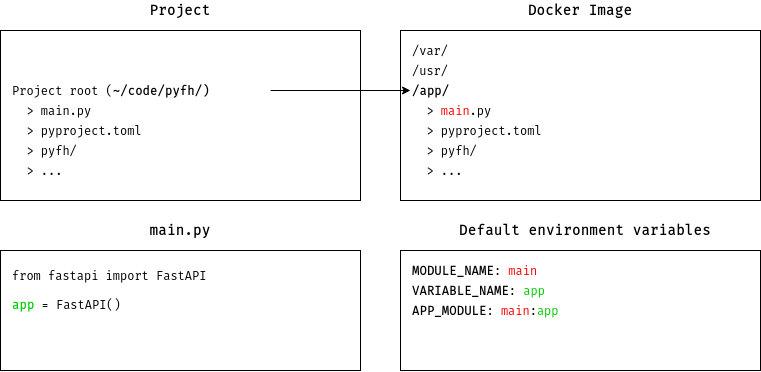
\includegraphics[width=0.7\textwidth]{img/docker_mapping.png}
    \caption{File mapping and environment variables}
\end{figure}

The \texttt{APP\_MODULE} variable is actually used by Gunicorn to launch the app. It is either deduced from \texttt{MODULE\_NAME} and \texttt{VARIABLE\_NAME} or overridden by the user.

\subsubsection{\texttt{docker-compose.yml}\label{preparations:dockercompose}}

Docker Compose allows you to define, execute, and manage a single-/multicontainer application using YAML files. In our case, apart from the FastAPI application, we're going to be using a PostgreSQL database (in its own conatiner) and a frontend application (we'll worry about that later). Let's look at our \texttt{docker-compose.yml}:

\begin{dockercode}

\end{dockercode}

\subsubsection{\texttt{.dockerignore}}

Dockerignore is to Docker what gitignore is to git. You don't want to include intermediate files in your image to save space, and you don't want sensitive data left behind as well. The rule of thumb is that you include everything you'd include in \texttt{.gitignore} plus a few more additions to reduce image size (e.g. \texttt{.git} folder).

\subsection{Technical details}

\subsubsection{On Gunicorn, Uvicorn and Nginx integration}

\subsubsection{Nginx: inside or outside of Docker?}

\subsubsection{Docker cache invalidation and command order}

\subsubsection{Parent and child image caveats in Docker}

\section{Domain Model}

\subsection{Creating entities}

\end{document}
